\documentclass[12pt,letterpaper]{article}


\newcommand{\studentname}{Ben Bassett}

\title{\textsc{Lab 08: Measuring Microwaves}}
\newcommand{\shorttitle}{Measuring Microwaves}

\newcommand{\course}{PHY310}
\newcommand{\labdate}{10-29-2024}

%------------------------------------------------------------------------------------------------------------

\usepackage[letterpaper,left=1in,right=1in,bottom=1in,top=1in]{geometry}
\usepackage{fancyhdr}
\usepackage{subfigure}
\usepackage{graphicx}
\usepackage{amsmath}
\usepackage{cleveref}
\usepackage{booktabs}
\usepackage[british]{babel}
\usepackage[square,comma,numbers,sort&compress]{natbib}
\usepackage{csvsimple}
\usepackage{graphicx}
\usepackage{pgfplotstable}
\usepackage{textcomp,gensymb}
\usepackage{array}
\usepackage{tabu}
\usepackage{multirow}
\usepackage{url}
\usepackage{lipsum}
\usepackage{dsfont}
\pgfplotsset{compat=1.9}% supress warning
\begin{document}

%------------------------------------------------------------------------------------------------------------

\setlength{\parindent}{1em}
\setlength{\parskip}{0.5em}
\author{\course~Lab Journal \\ \\ \studentname} % \,\& \labpartner}
\date{\labdate}

\renewcommand\abstractname{Summary}

\pagestyle{fancy}
\fancyhead{}
\fancyhead[l]{\course:~\shorttitle}
\fancyhead[r]{\studentname}
\fancyfoot{}
\fancyfoot[C]{\thepage}
\renewcommand{\headrulewidth}{0pt}
\renewcommand{\footrulewidth}{0pt}

\renewcommand\bibname{References}

%------------------------------------------------------------------------------------------------------------

\renewcommand\abstractname{Abstract}
\maketitle

% COMMENT IN IF ASKED TO SUBMIT REPORT WITH ABSTRACT
\begin{abstract}
In this lab we used 6 different methods to measure the frequency of leaking microwaves using a diode and various measurement devices. While we cannot easily perceive that kind of electromagnetic radiation with our eyes, it is often present in small quantities, and can be measured using our understanding of the fundamental attributes of waves. In this case, we used an aluminum plate to create standing waves, making the wavelength and hence frequency straightforward to measure. We used slightly different techniques to measure the distance of this cavity and the voltage across the diode, and compared our results, one of which was quite close to the actual frequency of the microwave.
\end{abstract}

% \section{Abstract}
% Why, what, and how?

\section{Experimental Setup}

Materials given were a microwave, aluminum plate, cup with water, diode, instrumentation amplifier, multimeter, paper, and a ruler. My general setup is illustrated in Figure \ref{fig:setup}.

\begin{figure}[h]
    \centering
    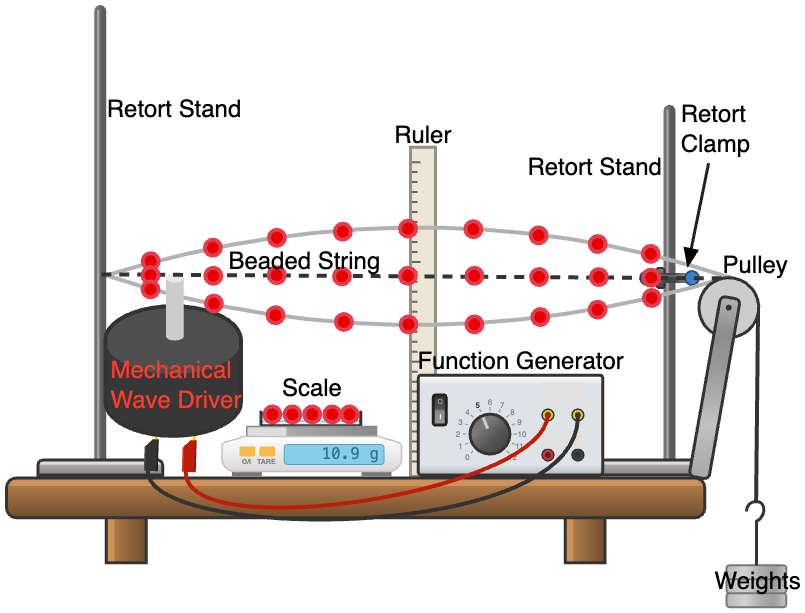
\includegraphics[width=6in]{images/setup.png}
    \caption{A diagram of my experimental setup}
    \label{fig:setup}
\end{figure}

% \pagebreak
\section{Procedure}

To setup, we placed the microwave on the table, taped down pieces of paper and made cm marks on it using the ruler. We then placed the aluminum plate vertically parallel to the door of the microwave. Between them we placed the diode, also parallel. We then attached cables to either end of the diode.

To ensure the microwaves had somewhere to go, we placed cups of ice water in the microwave, and ran each trial for 3 minutes then changed the water. We began by using the paper as our distance measurement. In our first trial, we used the DC voltage setting on our multimeter to attempt to see the voltage induced in the diode. We moved the plate back and forth to see where the voltage peaked, and marked that point as well as the amplitude at it. We repeated the same procedure on the AC voltage setting, then hooked up the diode to the instrumentation amplifier on the $\pm 20$ mV setting and graphed for 3 minutes as the microwave ran and we moved the plate back and forth.

We then repeated the same three trials, but this time with the motion detector setup behind the plate. For the multimeter readings, we just read the distance at the peak off the LabQuest, but graphed the distance along with voltage when using the instrumentation amplifier.

\section{Results}

While most of our values were written down by hand, you can see the peaks we observed with the motion detector and instrumentation amplifier along with a rolling average to see the exact locations of peaks in Figure \ref{fig:fit}. It's a bit messy because we moved the plate back and forth multiple times, so some distances have multiple values. Note that in the distance data the motion detector was placed behind the plate, so those values are inverted beginning at 30 cm away (e.g. the peak at 18 cm is actually a peak at 12 cm).

\begin{figure}[ht]
    \centering
    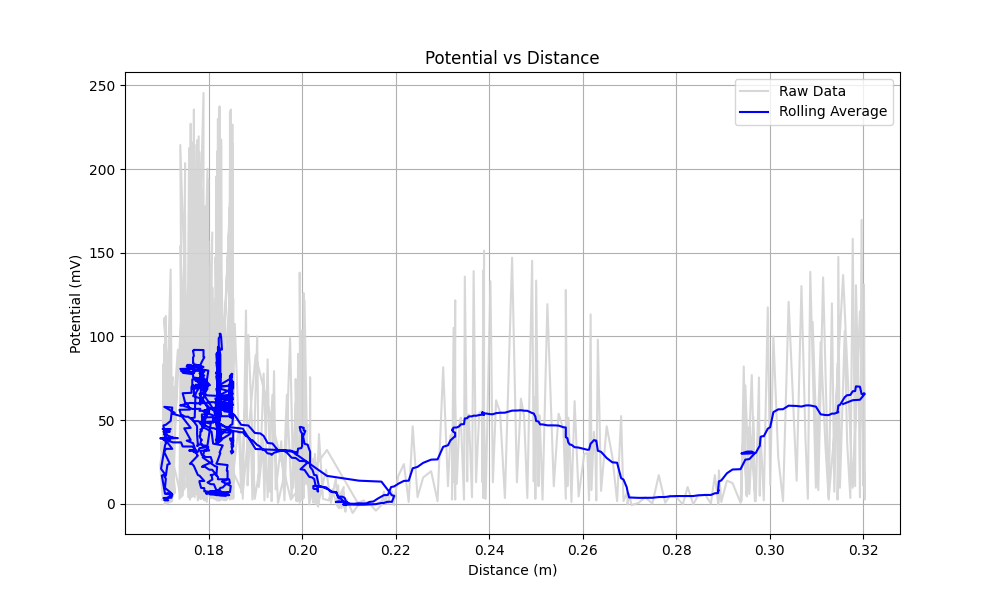
\includegraphics[width=6.5in]{images/potential_vs_distance.png}
    \caption{Voltage plotted as a function of distance from microwave}
    \label{fig:fit}
\end{figure}

Our compiled observed results for the locations of nodes of the standing waves are shown in Table \ref{tab:nodes}.

\begin{table}[h!]
    \centering
    \begin{tabular}{|c|c|c|c|c|}
        \hline
        Distance (cm) & DC Voltage & AC Voltage & Instrumentation Amplifier & Frequency (MHz) \\
        \hline
        \multicolumn{5}{|c|}{Paper} \\
        \hline
        30.0 ± 0.1 & 0.0078 ± 0.01 & - & - & 999 ± 3 \\
        \hline
        16.0 ± 0.1 & - & 0.016 ± 0.01 & - & 1870 ± 12 \\
        \hline
        22.0 ± 0.1 & - & 0.009 ± 0.01 & - & 1360 ± 6 \\
        \hline
        14.3 ± 0.1 & - & - & 0.0314 ± 0.01 & 2100 ± 15 \\
        \hline
        \multicolumn{5}{|c|}{Motion Sensor} \\
        \hline
        12.8 ± 0.1 & - & - & 0.2374 ± 0.01 & 2340 ± 18 \\
        \hline
        18.0 ± 0.1 & 0.007 ± 0.01 & - & - & 1670 ± 9 \\
        \hline
        14.0 ± 0.1 & 0.107 ± 0.01 & - & - & 2140 ± 15 \\
        \hline
        9.0 ± 0.1 & - & 0.015 ± 0.01 & - & 3330 ± 37 \\
        \hline
        16.0 ± 0.1 & - & 0.011 ± 0.01 & - & 1870 ± 12 \\
        \hline
    \end{tabular}
    \label{tab:nodes}
    \caption{Node locations and amplitude measurements for various methods}
\end{table}

We know that with waves, $v=\lambda f$. Since microwaves travel at the speed of light, and the speed of light in air is 299,792,458 m/s. Therefore, to compute the frequency of the microwave using our measurements for where nodes and standing waves were formed, we can say that 

\begin{equation}
    f=\frac{299792458 \frac{\text{m}}{\text{s}}}{\lambda \text{ m}}
\end{equation}

You can see I've computed this value using the equation and propagated errors in Table \ref{tab:nodes}. There was a significant amount of variety in our data due to the operation of other microwaves nearby, the very small voltage values the multimeter could read, the human inaccuracies in moving the plate exactly parallel back and forth at a smooth rate, and possible harmonics of the standing wave's nodes. However, using the motion sensor and instrumentation amplifier we see a node at 12.8 ± 0.1 cm, which yields a frequency of $\mathbf{2340 \pm 18} \textbf{ MHz}$.


\section{Conclusions}

We saw that with the best method of using the motion sensor and instrumentation amplifier we achieved a measurement of 2340 ± 18 MHz, which is favorably comparable to the frequency specified on the microwave of 2450 MHz. While there was a large amount of error in most of our measurements, it seems demonstrable that waves indeed behave as expected!


% \bibliographystyle{unsrtnat}
% \bibliography{references}

\end{document}
